\documentclass[journal,12pt,twocolumn]{IEEEtran}

\usepackage{setspace}
\usepackage{gensymb}
\singlespacing
\usepackage[cmex10]{amsmath}

\usepackage{amsthm}

\usepackage{mathrsfs}
\usepackage{txfonts}
\usepackage{stfloats}
\usepackage{bm}
\usepackage{cite}
\usepackage{cases}
\usepackage{subfig}

\usepackage{longtable}
\usepackage{multirow}

\usepackage{enumitem}
\usepackage{mathtools}
\usepackage{steinmetz}
\usepackage{tikz}
\usepackage{circuitikz}
\usepackage{verbatim}
\usepackage{tfrupee}
\usepackage[breaklinks=true]{hyperref}
\usepackage{graphicx}
\usepackage{tkz-euclide}

\usetikzlibrary{calc,math}
\usepackage{listings}
    \usepackage{color}                                            %%
    \usepackage{array}                                            %%
    \usepackage{longtable}                                        %%
    \usepackage{calc}                                             %%
    \usepackage{multirow}                                         %%
    \usepackage{hhline}                                           %%
    \usepackage{ifthen}                                           %%
    \usepackage{lscape}     
\usepackage{multicol}
\usepackage{chngcntr}

\DeclareMathOperator*{\Res}{Res}

\renewcommand\thesection{\arabic{section}}
\renewcommand\thesubsection{\thesection.\arabic{subsection}}
\renewcommand\thesubsubsection{\thesubsection.\arabic{subsubsection}}

\renewcommand\thesectiondis{\arabic{section}}
\renewcommand\thesubsectiondis{\thesectiondis.\arabic{subsection}}
\renewcommand\thesubsubsectiondis{\thesubsectiondis.\arabic{subsubsection}}


\hyphenation{op-tical net-works semi-conduc-tor}
\def\inputGnumericTable{}                                 %%

\lstset{
%language=C,
frame=single, 
breaklines=true,
columns=fullflexible
}
\begin{document}


\newtheorem{theorem}{Theorem}[section]
\newtheorem{problem}{Problem}
\newtheorem{proposition}{Proposition}[section]
\newtheorem{lemma}{Lemma}[section]
\newtheorem{corollary}[theorem]{Corollary}
\newtheorem{example}{Example}[section]
\newtheorem{definition}[problem]{Definition}

\newcommand{\BEQA}{\begin{eqnarray}}
\newcommand{\EEQA}{\end{eqnarray}}
\newcommand{\define}{\stackrel{\triangle}{=}}
\bibliographystyle{IEEEtran}
\raggedbottom
\setlength{\parindent}{0pt}
\providecommand{\mbf}{\mathbf}
\providecommand{\pr}[1]{\ensuremath{\Pr\left(#1\right)}}
\providecommand{\qfunc}[1]{\ensuremath{Q\left(#1\right)}}
\providecommand{\sbrak}[1]{\ensuremath{{}\left[#1\right]}}
\providecommand{\lsbrak}[1]{\ensuremath{{}\left[#1\right.}}
\providecommand{\rsbrak}[1]{\ensuremath{{}\left.#1\right]}}
\providecommand{\brak}[1]{\ensuremath{\left(#1\right)}}
\providecommand{\lbrak}[1]{\ensuremath{\left(#1\right.}}
\providecommand{\rbrak}[1]{\ensuremath{\left.#1\right)}}
\providecommand{\cbrak}[1]{\ensuremath{\left\{#1\right\}}}
\providecommand{\lcbrak}[1]{\ensuremath{\left\{#1\right.}}
\providecommand{\rcbrak}[1]{\ensuremath{\left.#1\right\}}}
\theoremstyle{remark}
\newtheorem{rem}{Remark}
\newcommand{\sgn}{\mathop{\mathrm{sgn}}}
\providecommand{\abs}[1]{\ensuremath{\left\vert#1\right\vert}}
\providecommand{\res}[1]{\Res\displaylimits_{#1}} 
\providecommand{\norm}[1]{\ensuremath{\left\lVert#1\right\rVert}}
%\providecommand{\norm}[1]{\lVert#1\rVert}
\providecommand{\mtx}[1]{\mathbf{#1}}
\providecommand{\mean}[1]{E\ensuremath{\left[ #1 \right]}}
\providecommand{\fourier}{\overset{\mathcal{F}}{ \rightleftharpoons}}
%\providecommand{\hilbert}{\overset{\mathcal{H}}{ \rightleftharpoons}}
\providecommand{\system}{\overset{\mathcal{H}}{ \longleftrightarrow}}
	%\newcommand{\solution}[2]{\textbf{Solution:}{#1}}
\newcommand{\solution}{\noindent \textbf{Solution: }}
\newcommand{\cosec}{\,\text{cosec}\,}
\providecommand{\dec}[2]{\ensuremath{\overset{#1}{\underset{#2}{\gtrless}}}}
\newcommand{\myvec}[1]{\ensuremath{\begin{pmatrix}#1\end{pmatrix}}}
\newcommand{\mydet}[1]{\ensuremath{\begin{vmatrix}#1\end{vmatrix}}}
\numberwithin{equation}{subsection}
\makeatletter
\@addtoreset{figure}{problem}
\makeatother
\let\StandardTheFigure\thefigure
\let\vec\mathbf
\renewcommand{\thefigure}{\theproblem}
\def\putbox#1#2#3{\makebox[0in][l]{\makebox[#1][l]{}\raisebox{\baselineskip}[0in][0in]{\raisebox{#2}[0in][0in]{#3}}}}
     \def\rightbox#1{\makebox[0in][r]{#1}}
     \def\centbox#1{\makebox[0in]{#1}}
     \def\topbox#1{\raisebox{-\baselineskip}[0in][0in]{#1}}
     \def\midbox#1{\raisebox{-0.5\baselineskip}[0in][0in]{#1}}
\vspace{3cm}
\title{Assignment 1}
\author{Vedala Sai Ashok - EE18BTECH11044}
\maketitle
\newpage
\bigskip
\renewcommand{\thefigure}{\theenumi}
\renewcommand{\thetable}{\theenumi}

Download all the C and Python codes from 
\begin{lstlisting}
wget https://github.com/hellblazer1/EE3025_A1/tree/master/codes
\end{lstlisting}
Download all the sound and data files from 
\begin{lstlisting}
wget https://github.com/hellblazer1/EE3025_A1/tree/master/data
\end{lstlisting}


\section{Digital Filter}
\begin{enumerate}[label=\thesection.\arabic*,ref=\thesection.\theenumi]
\item
\label{prob:1_1}
Download the sound file from  
\begin{lstlisting}
wget https://raw.githubusercontent.com/gadepall/EE1310/master/filter/codes/Sound_Noise.wav
\end{lstlisting}
\item
\label{prob:1_2}
Write the python code for removal of out of band noise and execute the code.
\\
\solution
\lstinputlisting{./codes/1_2.py}
\end{enumerate}
\section{Difference equation}
\begin{enumerate}[label=\thesection.\arabic*,ref=\thesection.\theenumi]
\item
\label{prob:2_1}
Write the difference equation of the above Digital filter obtained in problem \ref{prob:1_2}.
\\
\solution
\begin{align}
\label{eq:2_1}
 \sum _{m=0}^{M}a\brak{m}y\brak{n-m}=\sum _{k=0}^{N}b\brak{k}x\brak{n-k}
\end{align}
The resultant difference equation is given by \eqref{eq:2_2}
\begin{align}
\label{eq:2_2}
y(n) - 2.51946y(n-1) + 2.56083y(n-2) - 
\nonumber\\
1.20623y(n-3) + 0.22012y(n-4) = 0.00345x(n) + 
\nonumber\\
0.01381x(n-1) + 0.02072x(n-2) +
\nonumber \\
0.01381x(n-3) + 0.00345x(n-4)
\end{align}
\item
\label{prob:2_2}
Sketch x(n) and y(n).
\\
\solution
The following python code generates .dat file for Sound\_Noise.wav
\begin{lstlisting}
codes/2_1.py
\end{lstlisting}
The following C code takes the above generated .dat file as input and computes output from the difference equation and writes it into a .dat file
\begin{lstlisting}
codes/2_2.c
\end{lstlisting}
The following code plots Fig. \ref{fig:2_2}.
\begin{lstlisting}
codes/2_2.py
\end{lstlisting}

\begin{figure}[!ht]
\begin{center}
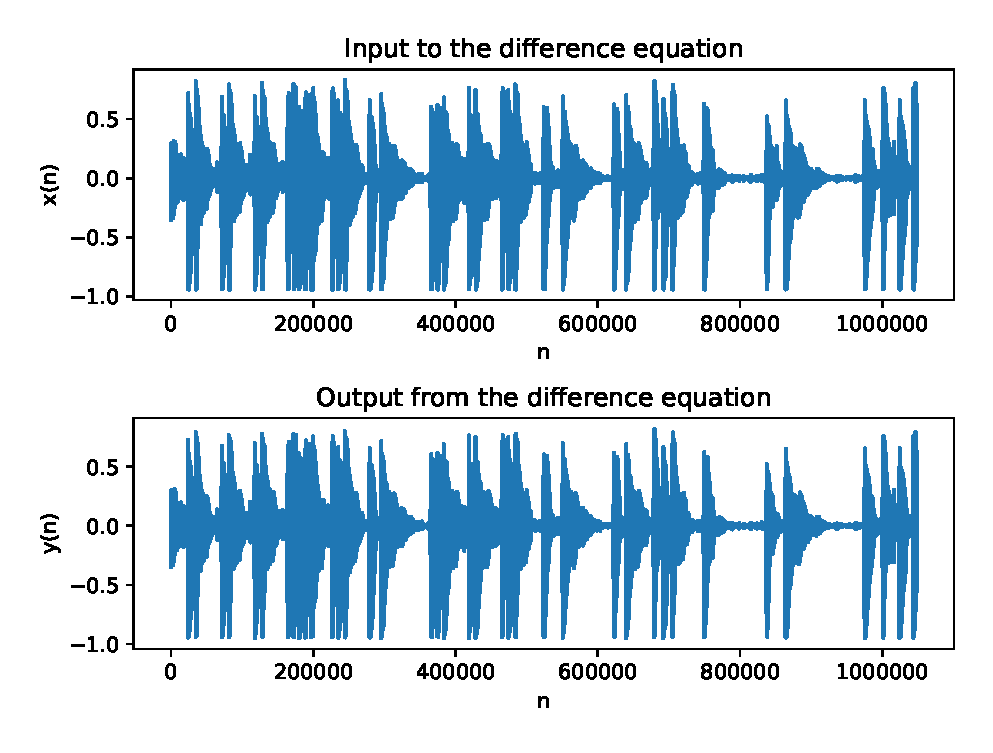
\includegraphics[width=\columnwidth]{./figs/2_2}
\end{center}
\captionof{figure}{}
\label{fig:2_2}	
\end{figure}
\end{enumerate}

%--------------------------------------------------------------------------------------------------------

\section{Z-transform}
\begin{enumerate}[label=\thesection.\arabic*,ref=\thesection.\theenumi]
\item
\label{prob:3_1}

The Z-transform of $x(n)$ is defined as
\begin{align}
\label{eq:3_1}
X(z)={\mathcal {Z}}\{x(n)\}=\sum _{n=-\infty }^{\infty }x(n)z^{-n}
\end{align}
%
Show that
\begin{equation}
\label{eq:3_2}
{\mathcal {Z}}\{x(n-1)\} = z^{-1}X(z)
\end{equation}
and find
\begin{equation}
	{\mathcal {Z}}\{x(n-k)\} 
\end{equation}
\\
\solution From \eqref{eq:3_1},
\begin{align}
{\mathcal {Z}}\{x(n-1)\} &=\sum _{n=-\infty }^{\infty }x(n-1)z^{-n}
\\
&=\sum _{n=-\infty }^{\infty }x(n)z^{-n-1} = z^{-1}\sum _{n=-\infty }^{\infty }x(n)z^{-n}
\end{align}
resulting in \eqref{eq:3_2}. Similarly, it can be shown that
%
\begin{equation}
\label{eq:3_3}
	{\mathcal {Z}}\{x(n-k)\} = z^{-k}X(z)
\end{equation}
\item Find
%
\begin{equation}
H(z) = \frac{Y(z)}{X(z)}
\end{equation}
%
from  \eqref{eq:2_2} assuming that the $Z$-transform is a linear operation.
\\
\solution  Applying \eqref{eq:3_3} on \eqref{eq:2_2} we get,
\begin{align}
\begin{split}
H(z) &= \frac{Y(z)}{X(z)}                
\\
&=\frac{b[0]+b[1]z^{-1}+b[2]z^{-2}+b[3]z^{-3}+b[4]z^{-4}}{a[0]+a[1]z^{-1}+a[2]z^{-2}+a[3]z^{-3}+a[4]z^{-4}}
\label{eq:freq_resp}
\end{split}
\end{align}
where
\begin{align}
\vec{a} &= \myvec{1&-2.52&2.56&-1.206&0.22013}\\
\vec{b} &=\myvec{0.00345&0.0138&0.020725&0.0138& 0.00345}
\end{align}
%
\item 
Let
\begin{equation}
H\brak{e^{\j w}} = H\brak{z = e^{\j w}}.
\end{equation}
Plot $\abs{H\brak{e^{\j w}}}$.
\\
\solution
The following code plots Fig. \ref{fig:3_1}.
\begin{lstlisting}
codes/3_1.py
\end{lstlisting}
\begin{figure}[!ht]
\centering
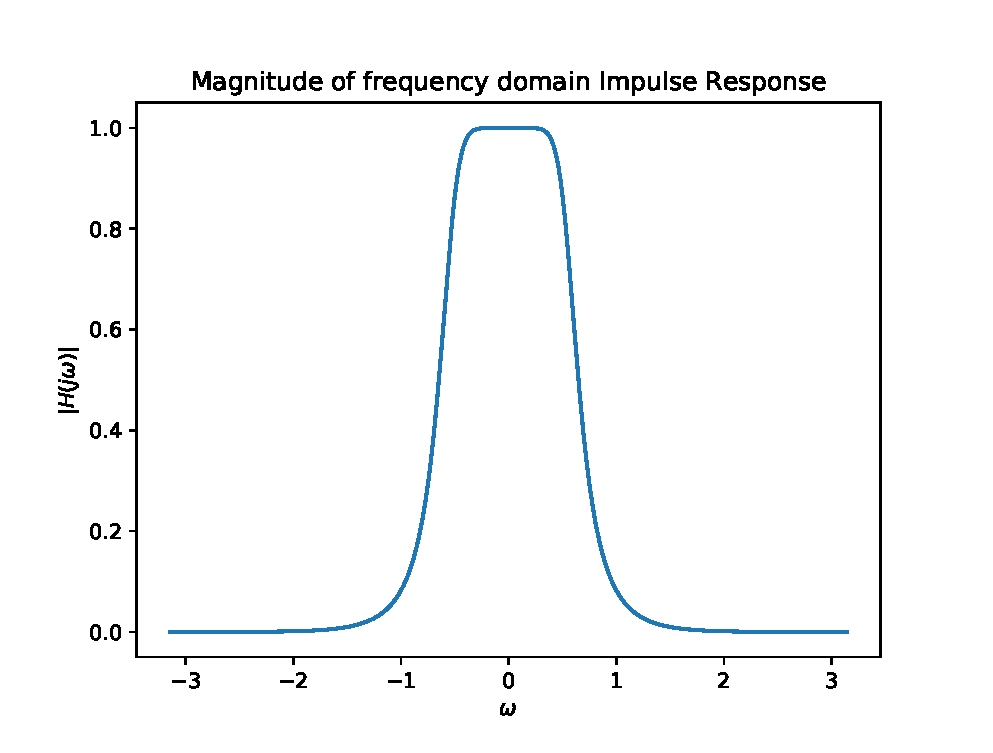
\includegraphics[width=\columnwidth]{./figs/3_1}
\caption{$\abs{H\brak{e^{\j w}}}$}
\label{fig:3_1}
\end{figure}
\end{enumerate}

%-------------------------------------------------------------------------------------------------
\section{Impulse Response}
\begin{enumerate}[label=\thesection.\arabic*,ref=\thesection.\theenumi]
\item
Sketch h(n).
\label{prob:4_1}
\\
\solution
h(n) is the impulse response of the system which means for an impulse input $\delta(n)$, the output of the system is h(n). Hence, by substituting $x(n)= \delta(n)$ in Eq. \eqref{eq:2_2} we can get h(n) of the system.
The following C code computes $h(n)$ from the difference equation \eqref{eq:2_2} and writes it into a .dat file
\begin{lstlisting}
codes/4_1.c
\end{lstlisting}
The following code plots Fig. \ref{fig:4_1} from the .dat file.
\begin{lstlisting}
codes/4_1.py
\end{lstlisting}
\begin{figure}[!ht]
\centering
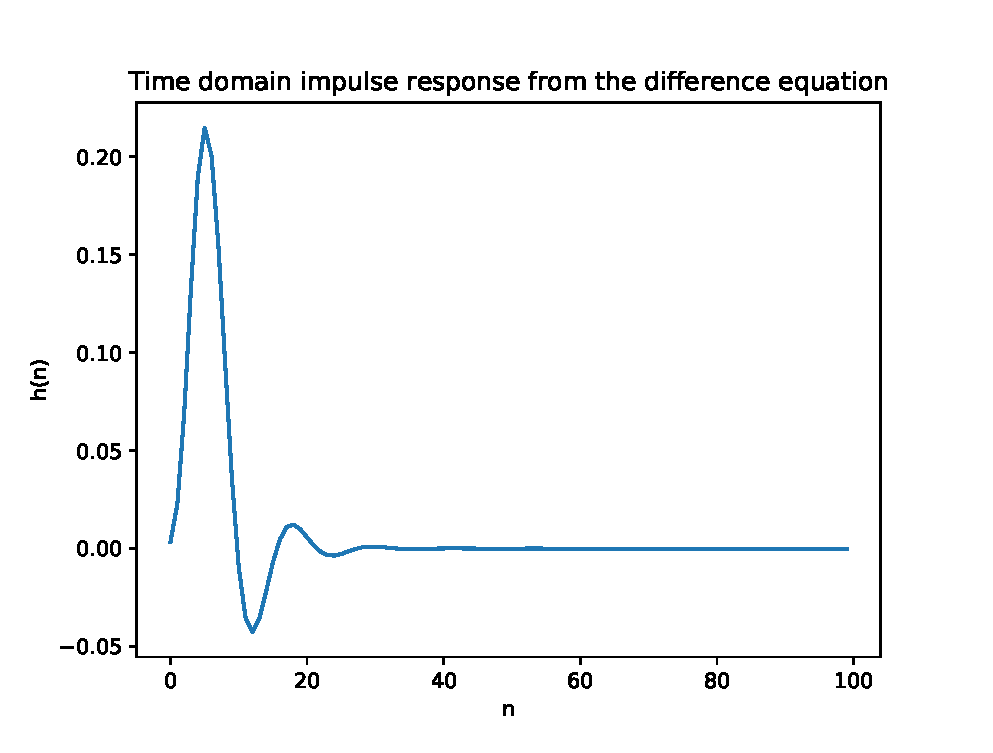
\includegraphics[width=\columnwidth]{./figs/4_1}
\caption{$h(n)$}
\label{fig:4_1}
\end{figure}
\item Check whether h(n) obtained is stable.
\\
\solution
For a system to be stable, output should be bounded for any bounded input. This is known as BIBO stability.
Since x(n) is bounded (the input), let $B_{x}$ be some finite value
\begin{equation}
\abs{y(n)} \leq B_{x}\sum_{-\infty}^{\infty} \abs{x(n-k)}
\label{eq:4_1}
\end{equation}
Using convolution,
\begin{align}
y(n)=h(n) * x(n) = x(n) * h(n)
\end{align}
Equation \eqref{eq:4_1} implies,
\begin{equation}
\abs{y(n)} = \abs{\sum_{-\infty}^{\infty} h(k)x(n-k)}
\end{equation}
\begin{equation}
\abs{y(n)} \leq \sum_{-\infty}^{\infty} \abs{h(k)}\abs{x(n-k)}
\end{equation}
Let $B_{x}$ be the maximum value x(n-k) can take, then
\begin{equation}
\abs{y(n)} \leq B_{x}\sum_{-\infty}^{\infty} \abs{h(k)}
\end{equation}
If
\begin{equation}
\sum_{-\infty}^{\infty} \abs{h(k)} < \infty
\end{equation}
Then
\begin{equation}
\abs{y(n)} \leq B_{y} < \infty
\end{equation}
Therefore we can say that y(n) is bounded if x(n) and h(n) are bounded.
Since the audio input is bounded, the system is said to be stable if h(n) is also bounded
\begin{equation}
\sum_{n=-\infty}^{n=-\infty} \abs{h(n)}<\infty
\end{equation}
The above equation can be re written as,
\begin{equation}
\sum_{n=-\infty}^{n=\infty} \abs{h(n)z^{-n}}_{\abs{z}=1}<\infty
\end{equation}
\begin{equation}
\sum_{n=-\infty}^{n=-\infty} \abs{h(n)} \abs{z^{-n}}_{\abs{z}=1}<\infty
\end{equation}
From Triangle inequality,
\begin{equation}
\abs{\sum_{n=-\infty}^{n=-\infty} h(n)z^{-n}}_{\abs{z}=1}<\infty
\end{equation}
\begin{equation}
\implies \abs{H(z)}_{\abs{z}=1} < \infty
\end{equation}
For the system to be stable, the Region of Convergence(ROC) should include the unit circle.
Since, h(n) is right sided the ROC is outside the outer most pole. From the equation \eqref{eq:freq_resp}, poles and zeros can be found by equating denominator and numerator to zero respectively.
Poles of the given transfer equation are:
\begin{equation}
\begin{split}
z(approx) = 0.69786 \pm 0.4132i,
\\
 0.56187 \pm 0.13779i
\end{split}  
\end{equation}
From the above poles, we can see that that the ROC of the system is
\begin{align}
\abs{z}&>\sqrt{0.69786^{2}+0.4132^{2}}
\\
\abs{z}&>0.811
\label{eq:4_2}
\end{align}
The following code plots the Fig. \ref{fig:4_2}
\begin{lstlisting}
codes/4_2.py
\end{lstlisting}
\begin{figure}[!ht]
\centering
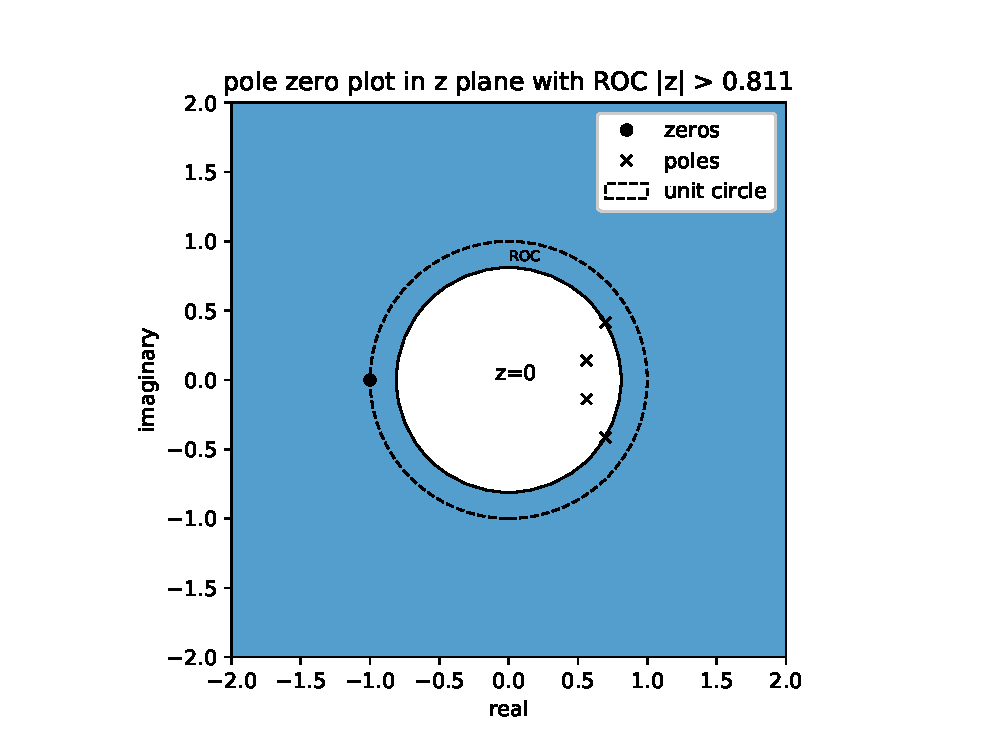
\includegraphics[width=\columnwidth]{./figs/4_2}
\caption{$ROC$}
\label{fig:4_2}
\end{figure}
From Equation \eqref{eq:4_2} and Fig. \ref{fig:4_2} we can observe that ROC of the system includes unit circle $\abs{z}=1$. Therefore, the given IIR filter is stable, since h(n) is absolutely summable.
\\
\textbf{Verification}:-
Given bounded input x(n) (audio sample) and system difference equation \eqref{eq:2_2}
From Fig. \ref{fig:2_2} we can see that the maximum value of x(n) is 0.8311 and minimum value is around -0.9417.
Similarly from Fig. \ref{fig:2_2} we can also observe that the maximum value of y(n) is 0.8362 and minimum value is -0.97 and it tends to zero after the length of signal.
We can conclude that for the bounded input x(n), the output
y(n) is bounded. Therefore, the system is BIBO stable. Also from Fig. \ref{fig:4_1}, we can observe that h(n) is converging to zero.
\\
\item Compute filtered output using convolution formula with h(n) obtained in \ref{prob:4_1}
%
\begin{equation}
\label{eq:4_3}
y(n) = x(n)*h(n) = \sum_{n=-\infty}^{\infty}x(k)h(n-k)
\end{equation}
\solution The following code plots Fig. \ref{fig:4_3} where $y(n)$ is computed using convolution.
%
\begin{lstlisting}
codes/4_3.py
\end{lstlisting}
\begin{figure}[!ht]
\centering
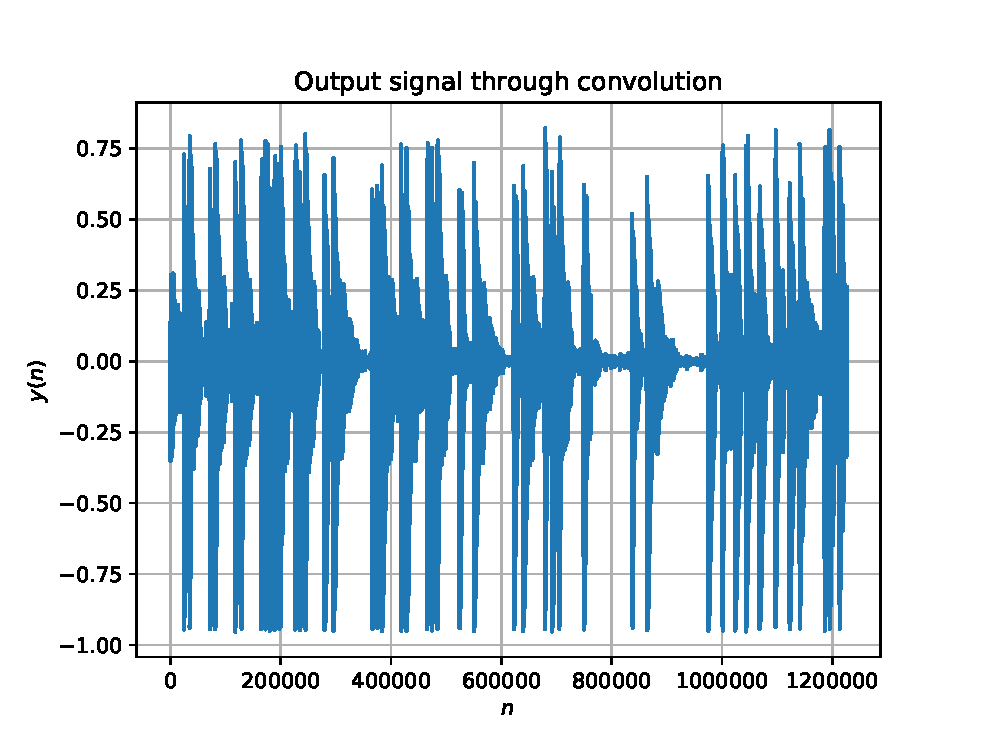
\includegraphics[width=\columnwidth]{./figs/4_3}
\caption{$y(n)$ through convolution}
\label{fig:4_3}
\end{figure}
We can observe that the output obtained in the Fig. \ref{fig:4_3} is same as y(n) obtained in Fig. \ref{fig:2_2}.

\end{enumerate}
%----------------------------------------------------------------------------------------
\section{FFT and IFFT}
\begin{enumerate}[label=\thesection.\arabic*
,ref=\thesection.\theenumi]
\item Compute
\begin{align}
        X(k) \triangleq \sum_{n=0}^{N-1} x(n) e^{-j 2 \pi k n / N}, \quad k=0,1, \ldots, N-1
\end{align}
and $H(k)$ using h(n).
\\
\solution
For the given IIR system with audio sample as x(n) and h(n) as impulse response where h(n) is obtained in section \ref{prob:4_1} 
DFT of the Input Signal $x(n)$ is 
\begin{align}
    X(k) \triangleq \sum_{n=0}^{N-1} x(n) e^{-j 2 \pi k n / N}, \quad k=0,1, \ldots, N-1
\end{align}
DFT of the Impulse Response $h(n)$ is 
\begin{align}
    H(k) \triangleq \sum_{n=0}^{N-1} h(n) e^{-j 2 \pi k n / N}, \quad k=0,1, \ldots, N-1
\end{align}
The following C code computes FFT of $x(n)$ and $h(n)$ using recursive sub-block approach. It also computes IFFT of Y(k) and creates a .dat file.
\begin{lstlisting}
codes/5_1.c
\end{lstlisting}
The following code plots FFTs of $x(n)$ and $h(n)$ from the .dat files created by the above C code.
\begin{lstlisting}
codes/5_1.py
\end{lstlisting}
Magnitude plots of $|X(k)|$ and $|H(k)|$
\begin{figure}[!ht]
\centering
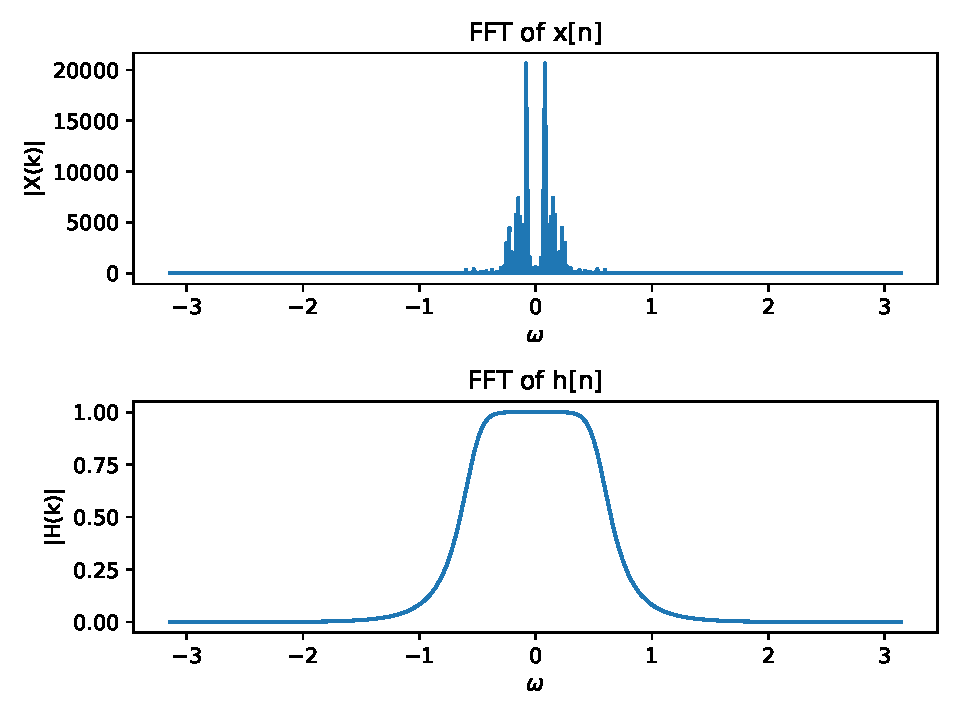
\includegraphics[width=\columnwidth]{./figs/5_1}
\caption{$X(k) and H(k)$}
\label{fig:5_1}
\end{figure}
\item From
\begin{equation}
Y(k) = X(k)H(k)
\end{equation}
Compute
\begin{equation}
y(n) \triangleq \sum_{k=0}^{N-1} Y(k) e^{j 2 \pi k n / N}, \quad n=0,1, \ldots, N-1
\end{equation}
\\
\solution
The following code plots Fig.\ref{fig:5_2}
\begin{lstlisting}
codes/5_2.py
\end{lstlisting}
\begin{figure}[!ht]
\centering
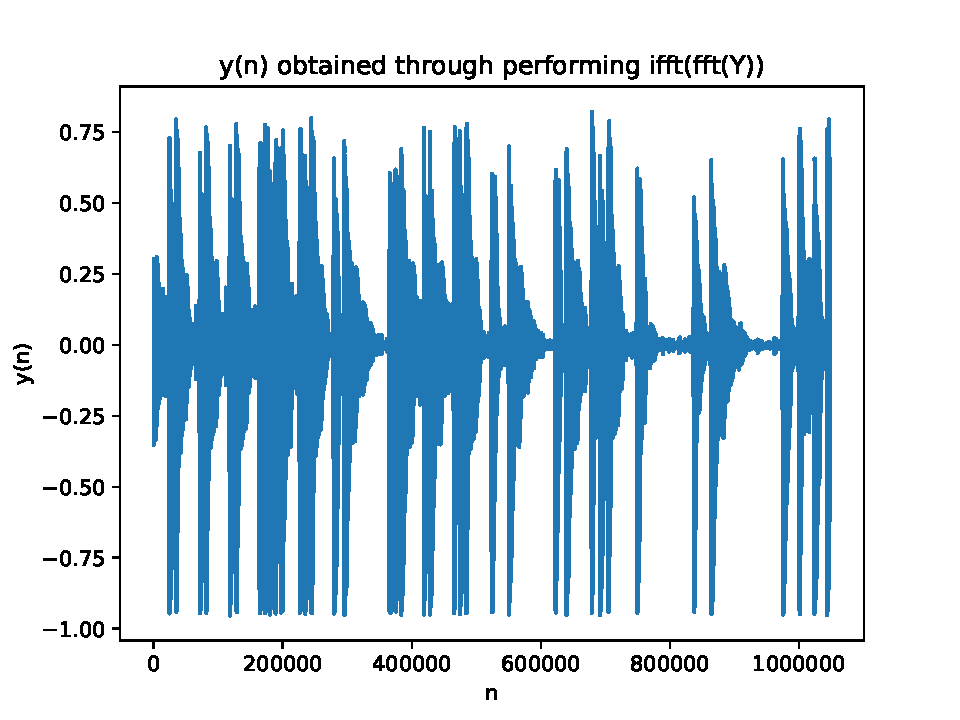
\includegraphics[width=\columnwidth]{./figs/5_2}
\caption{$y(n)$}
\label{fig:5_2}
\end{figure}
We can observe from the Fig. \ref{fig:5_2} that it is same as the y(n) observed in Fig.\ref{fig:2_2}
\end{enumerate}
\end{document}

